One can see the statistical results of the experiments in Figs. \ref{default_high}, \ref{default_max}, and \ref{high_max}.
The graphs can be seen in Figs. \ref{default_best_avg}, \ref{high_best_avg}, and \ref{max_best_avg}.
To run these experiments one simply needs to run either the \texttt{run.sh} shell script or the Python driver located in the source directory called \texttt{driver.py}.
The shell script just wraps the Python script and is there simply because it is required in the specifications.

\begin{figure}[H]
    \centering
    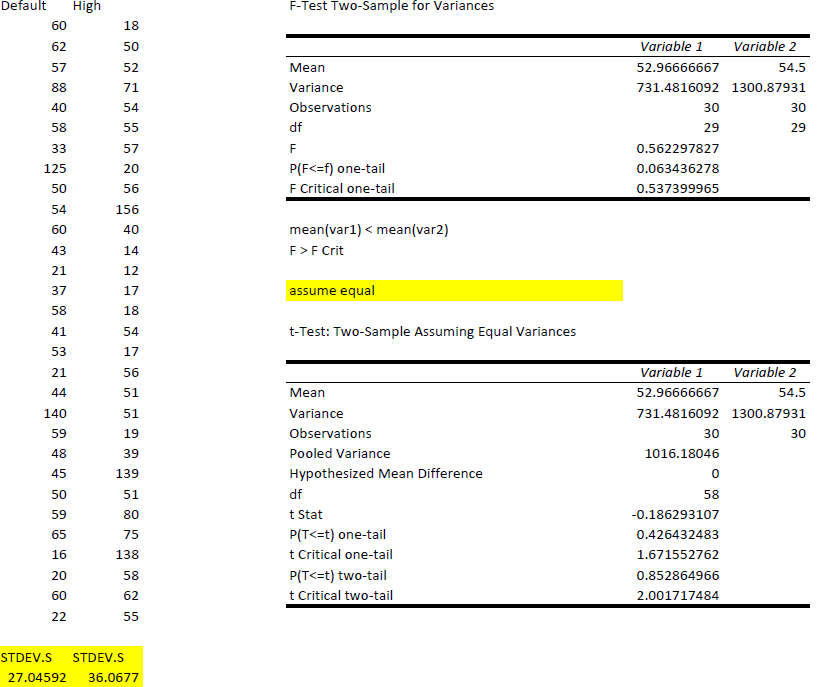
\includegraphics[width=.8\linewidth]{images/stats/default_high.png}
    \caption{Statistical Analysis for the Default Configuration versus the High Configuration}
    \label{default_high}
\end{figure}

\begin{figure}[H]
    \centering
    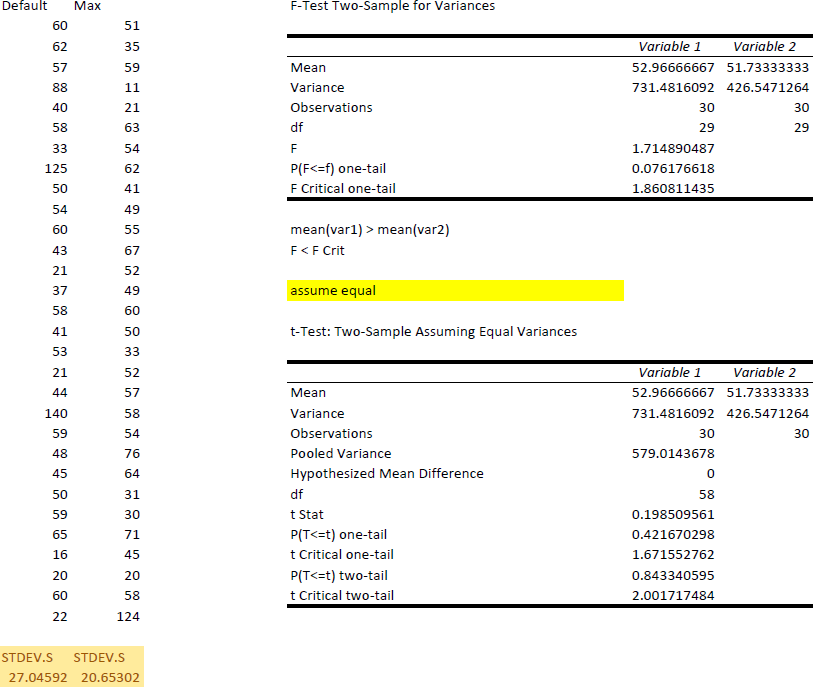
\includegraphics[width=.8\linewidth]{images/stats/default_max.png}
    \caption{Statistical Analysis for the Default Configuration versus the Max Configuration}
    \label{default_max}
\end{figure}

\begin{figure}[H]
    \centering
    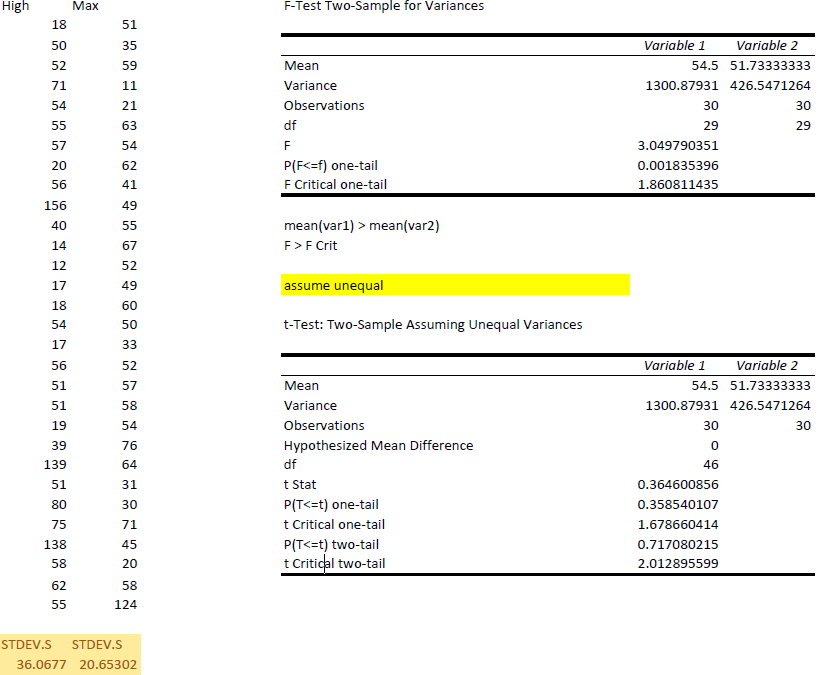
\includegraphics[width=.8\linewidth]{images/stats/high_max.png}
    \caption{Statistical Analysis for the High Configuration versus the Max Configuration}
    \label{high_max}
\end{figure}

\begin{figure}[H]
    \centering
    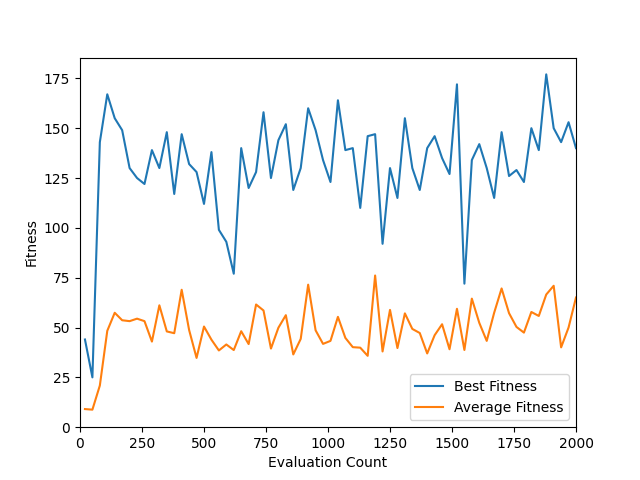
\includegraphics[width=.8\linewidth]{images/graphs/default_config_best_avg.png}
    \caption{Graph of Default Configuration best fitness per generation versus average fitness per generation}
    \label{default_best_avg}
\end{figure}

\begin{figure}[H]
    \centering
    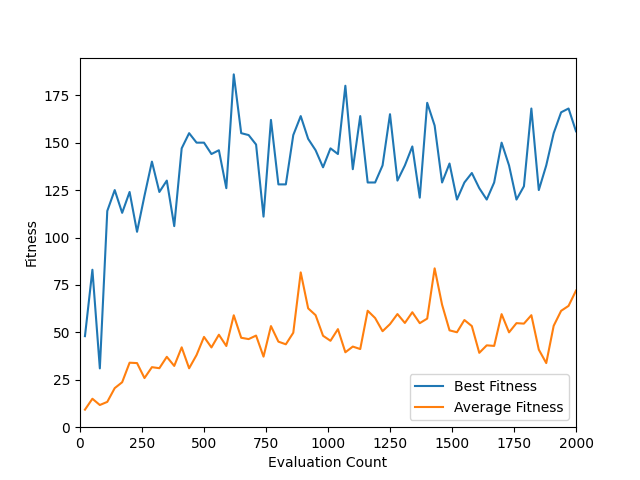
\includegraphics[width=.8\linewidth]{images/graphs/high_config_best_avg.png}
    \caption{Graph of High Configuration best fitness per generation versus average fitness per generation}
    \label{high_best_avg}
\end{figure}

\begin{figure}[H]
    \centering
    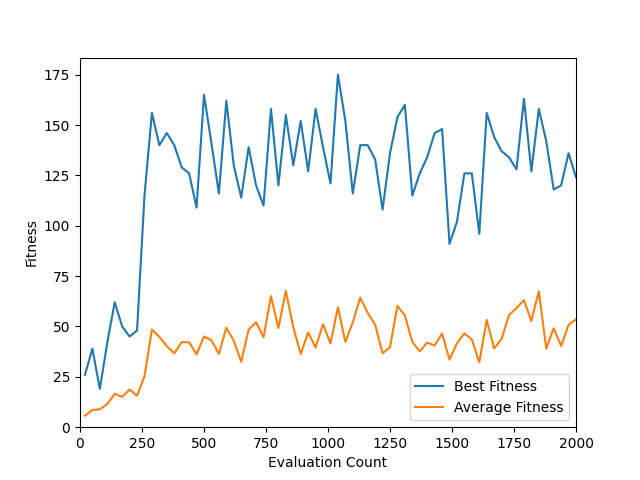
\includegraphics[width=.8\linewidth]{images/graphs/max_config_best_avg.png}
    \caption{Graph of Max Configuration best fitness per generation versus average fitness per generation}
    \label{max_best_avg}
\end{figure}